\documentclass[leqno]{article}
\usepackage[utf8x]{inputenc}
\usepackage[T1]{fontenc}
\usepackage{amsfonts}
\usepackage{enumerate}
\author{Colin Roberts}
\title{MATH 545, Homework 5}
\usepackage[left=3cm,right=3cm,top=3cm,bottom=3cm]{geometry}
\usepackage{amsmath}
\usepackage[thmmarks, amsmath, thref]{ntheorem}
%\usepackage{kbordermatrix}
\usepackage{mathtools}
\usepackage{color}
\usepackage{hyperref}
\usepackage{tikz-cd}
\usepackage{float}

\theoremstyle{nonumberplain}
\theoremheaderfont{\itshape}
\theorembodyfont{\upshape:}
\theoremseparator{.}
\theoremsymbol{\ensuremath{\square}}
\newtheorem{proof}{Proof}
\theoremsymbol{\ensuremath{\square}}
\newtheorem{lemma}{Lemma}
\theoremsymbol{\ensuremath{\blacksquare}}
\newtheorem{solution}{Solution}
\theoremseparator{. ---}
\theoremsymbol{\mbox{\texttt{;o)}}}
\newtheorem{varsol}{Solution (variant)}

\newcommand{\id}{\mathrm{Id}}
\newcommand{\im}{\mathrm{im}}
\newcommand{\R}{\mathbb{R}}
\newcommand{\N}{\mathbb{N}}
\newcommand{\Z}{\mathbb{Z}}

\newcommand{\End}{\mathrm{End}}

% Matlab code
\usepackage{listings}
\usepackage{color} %red, green, blue, yellow, cyan, magenta, black, white
\definecolor{mygreen}{RGB}{28,172,0} % color values Red, Green, Blue
\definecolor{mylilas}{RGB}{170,55,241}

\begin{document}
\maketitle
\begin{large}
\begin{center}
Solutions
\end{center}
\end{large}

%%%%%%%%%%%%%%%%%%%%%%%%%%%%%%%%%%%%%%%%%%%%%%%%%%%%%%%%%%%%%%%%%%%%%%%%%%%%%%%%%%%%%%%%%%%%%%%%%%%%%%%%%%%%%%%%%%%%%
%%%%%%%%%%%%%%%%%%%%%%%%%PROBLEM%%%%%%%%%%%%%%%%%%%%%%%%%%%%%%%%%%%%%%%%%%%%%%%%%%%%%%%%%%%%%%%%%%%%%%%%%%%%%%%%%%%%%%%%%%%%%%%%%%%%%%%%%%%%%%%%%%%%%%%%%%%%%%%%%%%%%%%%%%%%%%%%%%%%%%%%%%%%%%%%%%%%%%%%%%%%%%%%%%%%%%%%%%%%%%%%%%%%%%%%%%

\paragraph{Problem 1 (Solution of the heat equation on a rectangle).}
If the domain on which we want to solve the heat equation is a
rectangle, i.e., $\Omega=(0,L)\times(0,H) \subset \R^2$, then we had
derived that the solution of the heat equation with zero boundary
values,
\begin{align*}
\frac{\partial}{\partial t} u(x,y,t)
-
k
\Delta u(x,y,t)
&= 0
\qquad \text{for all $(x,y)\in\Omega$, $t>0$},
\\
u(x,y,t) &= 0
\qquad \text{for all $(x,y)\in\partial\Omega$, $t>0$},
\end{align*}
has the general form of a superposition of solutions we have found
through the separation of variables approach. Namely, that the
solution has the form
\begin{align*}
u(x,y,t)
=
\sum_{n=1}^\infty
\sum_{m=1}^\infty
A_{nm}
e^{-\left(\frac{n^2\pi^2}{L^2} + \frac{m^2\pi^2}{H^2}\right)t}
\sin\left(\frac{n\pi x}{L}\right)
\sin\left(\frac{m\pi y}{H}\right)
\end{align*}
Compute what values the coefficients $A_{nm}$ must take on so that the
solution $u(x,y,t)$ satisfies the following initial conditions:
\begin{align*}
u(x,y,0)
= u_0(x,y)
= \begin{cases}
  0 & \text{if $x<\frac L2$ and $y<\frac H2$, or if $x\ge\frac L2$ and
    $y\ge\frac H2$},
    \\
    1 & \text{otherwise}.
\end{cases}
\end{align*}


\begin{solution}
We have that
\[
A_{nm}=\frac{2}{L}\cdot \frac{2}{H} \int_{0}^H \int_0^L \sin \left(\frac{ n \pi x}{L}\right) \sin \left( \frac{m \pi y}{H}\right) u_0(x,y) dxdy.
\]
For our given $u_0(x,y)$, we then get
\[
A_{nm}=\frac{2}{L}\cdot \frac{2}{H} \left[ \int_{H/2}^H \int_0^{L/2} \sin \left(\frac{ n \pi x}{L}\right) \sin \left( \frac{m \pi y}{H}\right) dxdy + \int_{0}^{H/2} \int_{L/2}^L \sin \left(\frac{ n \pi x}{L}\right) \sin \left( \frac{m \pi y}{H}\right) dxdy\right].
\]
Evaluating these yields
\begin{align*}
    A_{nm}&=\frac{2}{L}\cdot \frac{2}{H} \left[ \frac{2HL \sin^2 \left(\frac{\pi n}{4}\right)\left( \cos \left(\frac{\pi m}{2}\right) - \cos (\pi m)\right)}{\pi^2 m n}\right. \\
    &\quad+\left. \frac{2HL \sin^2\left( \frac{\pi m}{4}\right)\left(\cos \left(\frac{\pi n}{2}\right)-\cos(\pi n)\right)}{\pi^2 m n}\right]
\end{align*}
\emph{I'm certain this could be simplified. However, I found no need to do that. I just used this form to plot it in Matlab.}
\end{solution}
\pagebreak


\paragraph{Problem 2 (Plotting 2d solutions).}
Given what you found in the previous problem, show a computer plot of
$u(x,y,t)$ for $t=0$ (and verify that it matches the initial
conditions) as well as for $t=0.1$, $t=0.5$, $t=1$, $t=10$.

Use $L=2,H=1,k=1$ for the constants that appear in the problem.

\begin{solution}
Here I used 30 terms for $n$ and for $m$.  Seemed to look good enough and was more time efficient. At around 50 terms each, the computer didn't seem to handle it.  Do you know why exactly that would be the case?  Memory? Plots follow:
\begin{figure}[h]
    \centering
    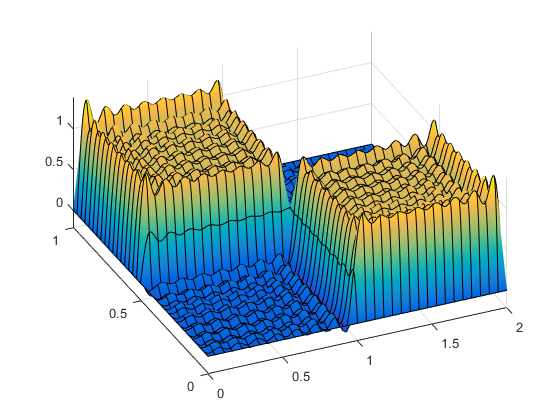
\includegraphics{problem_2_hw_5.png}
    \caption{For the case $t=0$.}
    \label{fig:my_label}
\end{figure}

\pagebreak

\begin{figure}[h]
    \centering
    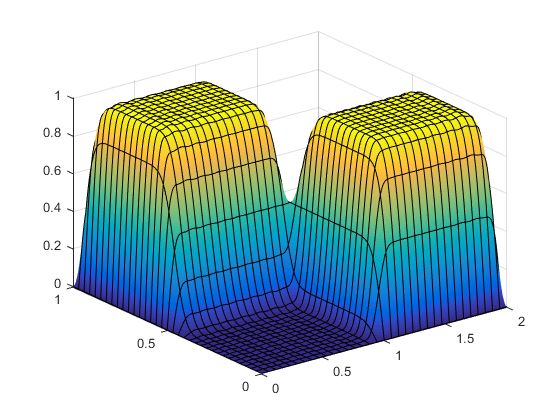
\includegraphics{problem_2_t=001_hw_5.png}
    \caption{For the case $t=0.001$. This was extra, but I wanted to see less of a change from initial conditions.}
    \label{fig:my_label}
\end{figure}

\pagebreak

\begin{figure}[h]
    \centering
    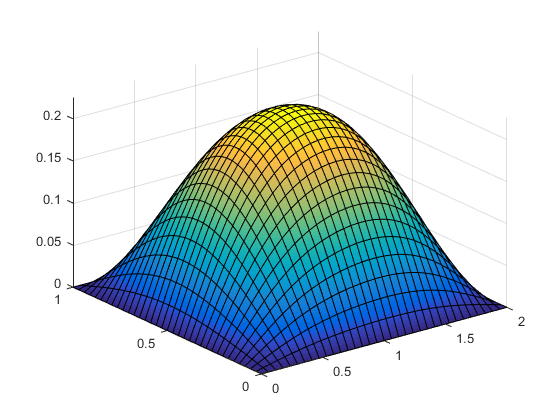
\includegraphics{problem_2_t=01_hw_5.png}
    \caption{For the case $t=0.1$. Note the scale on the axes.}
    \label{fig:my_label}
\end{figure}

\pagebreak

\begin{figure}[h]
    \centering
    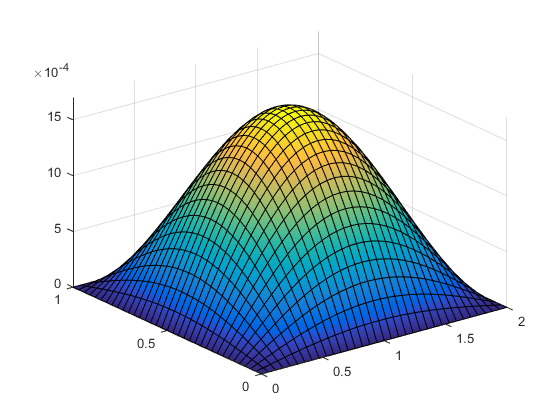
\includegraphics{problem_2_t=05_hw_5.png}
    \caption{For the case $t=0.5$. Note the scale on the axes.}
    \label{fig:my_label}
\end{figure}

\pagebreak

\begin{figure}[h]
    \centering
    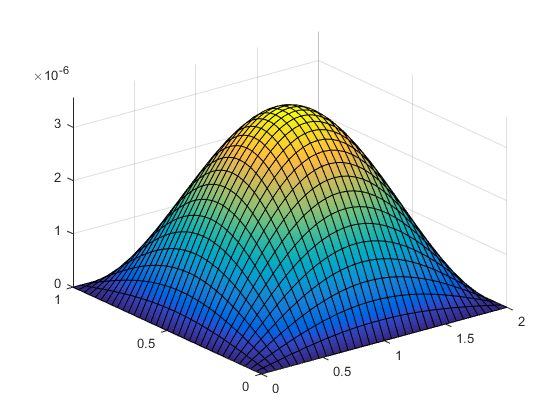
\includegraphics{problem_2_t=1_hw_5.png}
    \caption{For the case $t=1$. Note the scale on the axes.}
    \label{fig:my_label}
\end{figure}
    
\pagebreak
    
\begin{figure}[h]
    \centering
    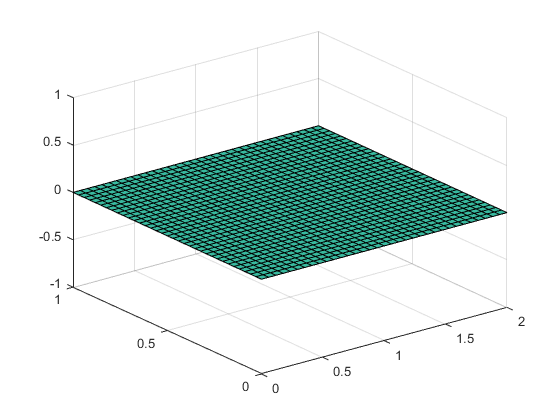
\includegraphics{problem_2_t=10_hw_5.png}
    \caption{For the case $t=10$.}
    \label{fig:my_label}
\end{figure}

\end{solution}
\pagebreak

\paragraph{Problem 3 (Fourier series).}
Derive the Fourier series on $[-\pi,\pi]$ of the function $f(x)=x$. From this
series, derive the Fourier series of $F(x)=x^2/2$ without using the formulas
$\frac 1L\int_{-L}^L F(x)\cos nx \; dx$ (and similar for the sine terms) to
compute the coefficients $A_0,A_n,B_n$ of the second series.

\begin{solution}
Note that $x$ is an odd function with average value $0$ on $[-\pi,\pi]$. It follows that all the cosine terms $A_n$ and $A_0$ are zero. Then we have
\[
B_n=\frac{1}{\pi}\int_{-\pi}^\pi x \sin{nx}dx.
\]
If we compute, we get
\begin{align*}
    B_n&=\frac{2\sin(\pi n)-2\pi n \cos (\pi n)}{\pi n^2}.
\end{align*}
We simplify this slightly to get
\begin{align*}
    B_n&=-\frac{2\cos (\pi n)}{n}\\
    &= \frac{2\cdot(-1)^{n+1}}{n}.
\end{align*}
Then the Fourier series is given by
\[
\overline{f}(x)=2\sum_{n=1}^\infty \frac{(-1)^{n+1}}{n}\sin (nx).
\]

Since this function is piecewise smooth, we can take the term-by-term antiderivative in order to find the Fourier series for $x^2/2.$ So we have
\[
2\frac{(-1)^{n+1}}{n} \int \sin (nx)dx &= 2 \frac{(-1)^{n+1}}{n}\cdot \frac{-\cos(n\pi)}{n} + C.
\]
Note that for the series to converge to finite values, we take $c=0$.   So,
\[
\overline{F}(x)=\overline{A}_0+ 2\sum_{n=1}^\infty \frac{(-1)^n}{n^2} \cos(n x).
\]
We want $\overline{F}(0)=0$, which means we have to find $\overline{A}_0$.  We plug in $x=0$ and then we have
\begin{align*}
\overline{F}(0)&=\overline{A}_0+2\sum_{n=1}^\infty \frac{(-1)^n}{n^2}\\
0&=\overline{A}_0-\frac{\pi^2}{6}\\
\implies \overline{A}_0&= \frac{\pi^2}{6}.
\end{align*}
Then, 
\[
\overline{F}(x)=\frac{\pi^2}{6}+ 2\sum_{n=1}^\infty \frac{(-1)^n}{n^2} \cos(n x).
\]
\end{solution}
\pagebreak

\paragraph{Problem 4 (Fourier series).}
Derive the Fourier series on $[-\pi,\pi]$ of the function $F(x)=x$ (it is the
same as in the previous problem). State whether you can derive the Fourier series of the
function $f(x)=1$ from it by differentiating each term in the series of $F(x)$
individually. State the Fourier series of $f(x)$.

\begin{solution}
The Fourier series for $F(x)$ comes from the previous problem. In particular,
\[
\overline{F}(x)=2\sum_{n=1}^\infty \frac{(-1)^{n+1}}{n}\sin (nx).
\]
The term by term derivative is 
\[
g(x)=2\sum_{n=1}^\infty (-1)^{n+1}\cos(nx).
\]
We cannot get the fourier series for $f(x)=1$ by term-by-term differentiation since $f$ is not periodic. Clearly the series we get from differentiating term-by-term doesn't even converge for each point.  Specifically, note that for $x=0$, the sequence of partial sums for the series oscillates between $-2$ and $2$.  This occurs more or less everywhere within the interval, from what I can see from the plots (in the future problem).

Instead, we find the Fourier series directly.  Note $f(x)$ is even, with average value $1$.  This means $A_0=1$ and all $B_n=0$.  Then
\begin{align*}
A_n &= \frac{1}{\pi} \int_{-\pi}^\pi \cos(nx)dx\\
&=0.
\end{align*}
So we have
\[
\overline{f}(x)=1.
\]
Again, we can see that this is not the same as the term-by-term derivative of $\overline{F}(x)$.
\end{solution}
\pagebreak

\paragraph{Problem 5 (Fourier series).} Generate computer plots of the
partial sums $\bar f_{10}(x) = a_0 + \sum_{n=1}^{10} a_n \cos(nx) +
\sum_{n=1}^{10} b_n \sin(nx)$
and $\bar F_{10}(x) = A_0 + \sum_{n=1}^{10} A_n \cos(nx) + \sum_{n=1}^{10} B_n \sin(nx)$
consisting of the first 10 terms for the Fourier series of the functions
$f(x)=1, F(x)=x$, where the Fourier series is calculated over the interval
$-\pi\ldots\pi$. Plot these Fourier series on the larger interval $-2\pi\ldots
2\pi$. 

Also generate a plot of the partial sum $g_{10}(x)=\sum_{n=1}^{10} -A_n n
\sin(nx) + \sum_{n=1}^{10} B_n n \cos(nx)$, using the coefficients
$A_n,B_n$ of the Fourier series of $F(x)=x$ (this is the term-by-term
differentiated Fourier series of $F(x)$ for which one may hope that it
matches $f(x)$.) Repeat this last part with
20, 30, 50, 100 terms instead of just 10. Do you think this series converges?

\begin{solution}
The plots follow: 

\begin{figure}[h]
    \centering
    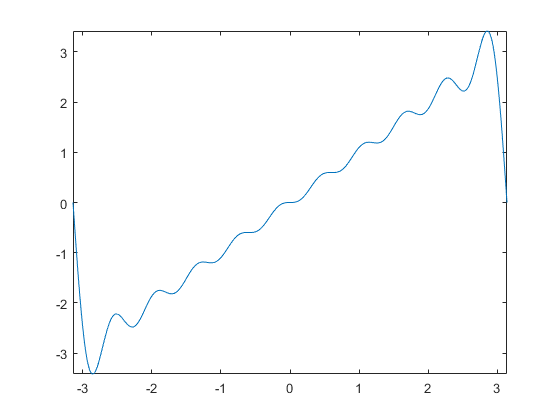
\includegraphics{problem_3_1_hw_5.png}
    \caption{Plot for $\overline{F}_{10}(x)$ on $[-\pi,\pi]$.}
    \label{fig:my_label}
\end{figure}
\pagebreak

\begin{figure}[h]
    \centering
    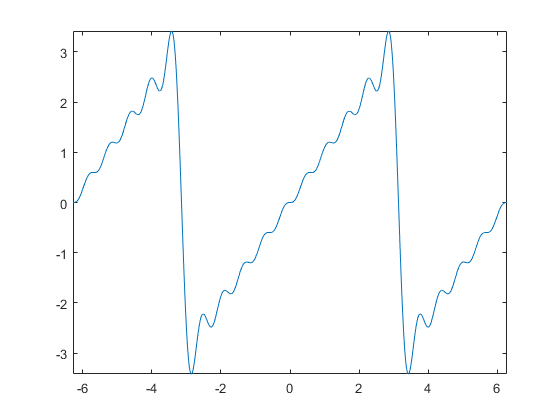
\includegraphics{problem_3_2_hw_5.png}
    \caption{Plot for $\overline{F}_{10}(x)$ on $[-2\pi,2\pi]$.}
    \label{fig:my_label}
\end{figure}
\pagebreak

\begin{figure}[h]
    \centering
    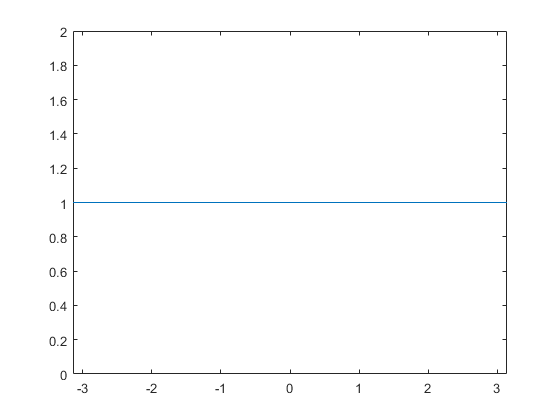
\includegraphics{problem_3_3_hw_5.png}
    \caption{Plot for $\overline{f}_{10}(x)$ on $[-\pi,\pi]$.}
    \label{fig:my_label}
\end{figure}
\pagebreak

\begin{figure}[h]
    \centering
    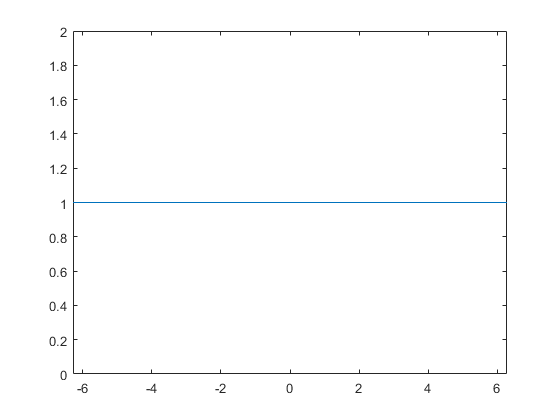
\includegraphics{problem_3_4_hw_5.png}
    \caption{Plot for $\overline{f}_{10}(x)$ on $[-2\pi,2\pi]$.}
    \label{fig:my_label}
\end{figure}
\pagebreak

\begin{figure}[h]
    \centering
    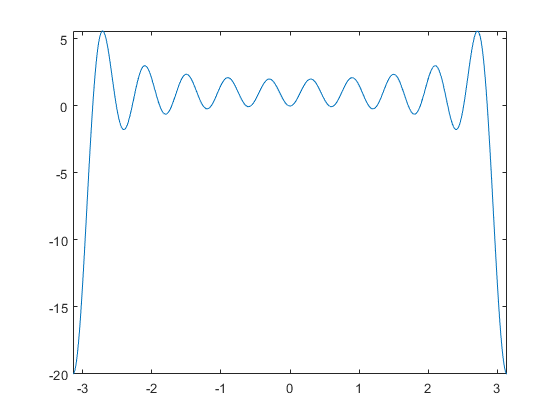
\includegraphics{problem_3_5_hw_5.png}
    \caption{Plot for $g_{10}(x)$ on $[-\pi,\pi]$.}
    \label{fig:my_label}
\end{figure}
\pagebreak

\begin{figure}[h]
    \centering
    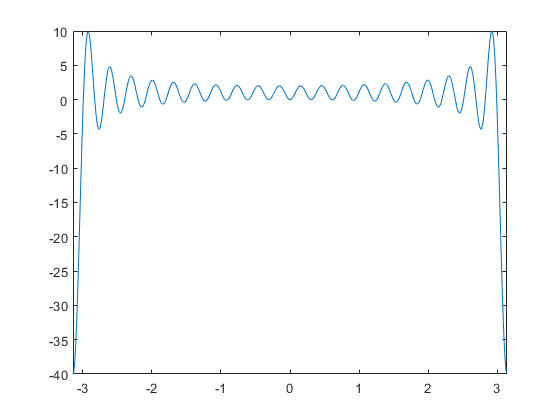
\includegraphics{problem_3_6_hw_5.png}
    \caption{Plot for $g_{20}(x)$ on $[-\pi,\pi]$.}
    \label{fig:my_label}
\end{figure}
\pagebreak

\begin{figure}[h]
    \centering
    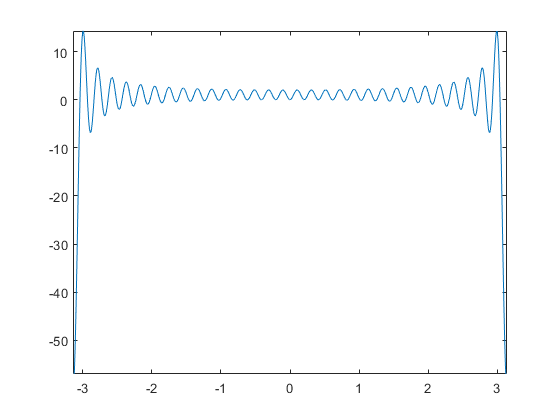
\includegraphics{problem_3_7_hw_5.png}
    \caption{Plot for $g_{30}(x)$ on $[-\pi,\pi]$.}
    \label{fig:my_label}
\end{figure}
\pagebreak

\begin{figure}[h]
    \centering
    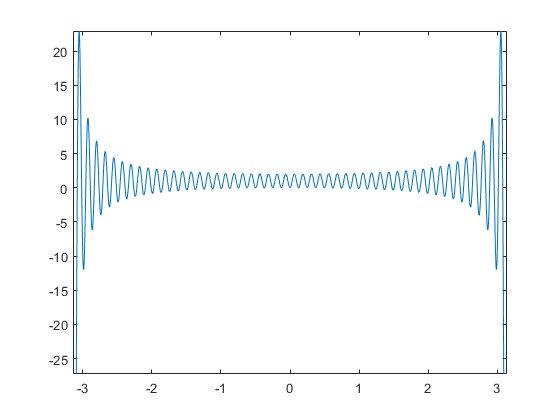
\includegraphics{problem_3_8_hw_5.png}
    \caption{Plot for $g_{50}(x)$ on $[-\pi,\pi]$.}
    \label{fig:my_label}
\end{figure}
\pagebreak

\begin{figure}[h]
    \centering
    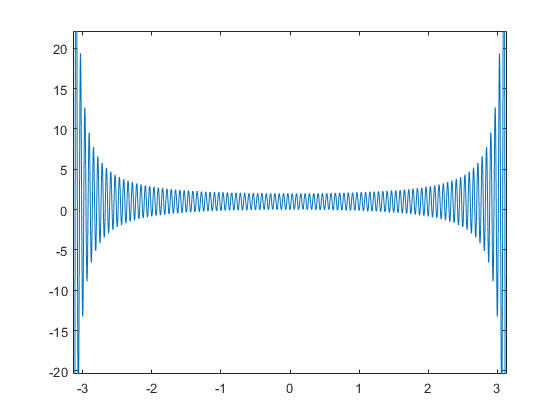
\includegraphics{problem_3_9_hw_5.png}
    \caption{Plot for $g_{100}(x)$ on $[-\pi,\pi]$.}
    \label{fig:my_label}
\end{figure}
\pagebreak

\end{solution}
\pagebreak

\paragraph{Problem 6 (Fourier series).} Calculate or look up the Fourier
series on the interval $-\pi\ldots\pi$ of the function
\begin{gather*}
  f(x) = \left\{{1\ \text{for $x>0$} \atop -1\ \text{for $x\le 0$}}\right.
\end{gather*}
Generate plots of the partial sums $f_N(x)=A_0 + \sum_{n=1}^N A_n
\cos(nx) + \sum_{n=1}^{N} B_n \sin(nx)$ consisting of the first $N$ terms, for each value
$N=2, 5, 10, 20, 50$. Try to determine the maximal difference $|f(x)-f_N(x)|$
numerically or graphically. We know that for $N\rightarrow \infty$,
$f_N(x)\rightarrow f(x)$ almost everywhere; is this consistent with your
results?

\begin{solution}
We have that $f(x)$ is odd with average value 0, so $A_0=0$ and $A_n=0$ for every $n$.  So we find
\[
B_n=\frac{1}{\pi}\left[-\int_{-\pi}^0 \sin(nx)dx+\int_{0}^\pi \sin(nx)dx\right].
\]
Evaluating, we get
\begin{align*}
    B_n&=\frac{2(1-\cos(\pi n))}{\pi n}\\
    &= \begin{cases}
    0 & n ~\textrm{even}\\
    \frac{4}{\pi n} & n ~\textrm{odd}
    \end{cases}
\end{align*}
So the Fourier series is
\[
\overline{f}(x)=\sum_{n=0}^\infty \frac{4}{\pi (2n+1)} \sin((2n+1)\pi).
\]
Graphically, we can see the maximal difference $|f(x)-f_N(x)|$ seems to be about $0.2$ to $0.3$.  However, for example, looking at $f_5$-$f_{50}$ we can see that point values with a large discrepancy ($0.1-0.3$) happen on smaller and smaller intervals.  In the limit, the set where this difference occurs will be one of measure zero.  This means we are fine to say that $f_N\to f$ almost everywhere.  Really, the notion pointwise convergence is not what we want to use here.  We are really looking for convergence in $L^2$ (or something related).

Here are the plots:
\begin{figure}[h!]
    \centering
    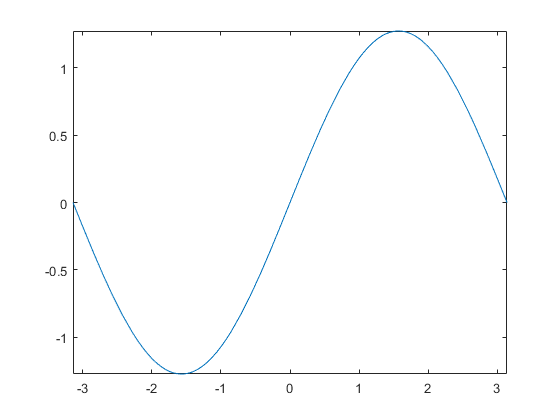
\includegraphics{problem_3_10_hw_5.png}
    \caption{$f_2(x)$ plotted on $[-\pi,\pi]$.}
    \label{fig:my_label}
\end{figure}
\pagebreak

\begin{figure}[h!]
    \centering
    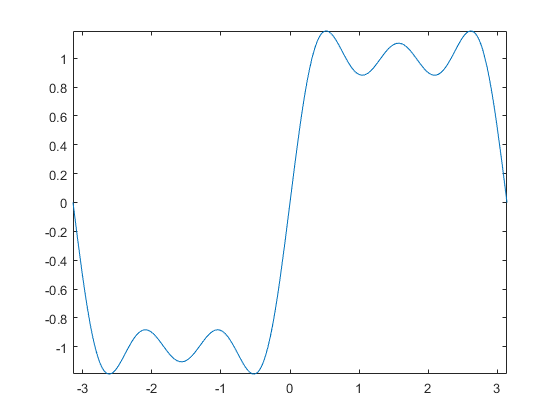
\includegraphics{problem_3_11_hw_5.png}
    \caption{$f_5(x)$ plotted on $[-\pi,\pi]$.}
    \label{fig:my_label}
\end{figure}
\pagebreak

\begin{figure}[h!]
    \centering
    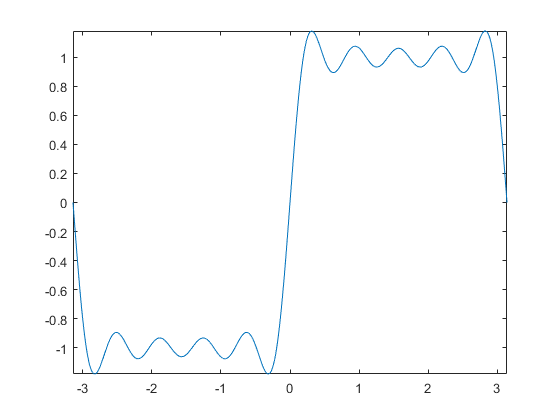
\includegraphics{problem_6_f10.png}
    \caption{$f_{10}(x)$ plotted on $[-\pi,\pi]$.}
    \label{fig:my_label}
\end{figure}
\pagebreak

\begin{figure}[h!]
    \centering
    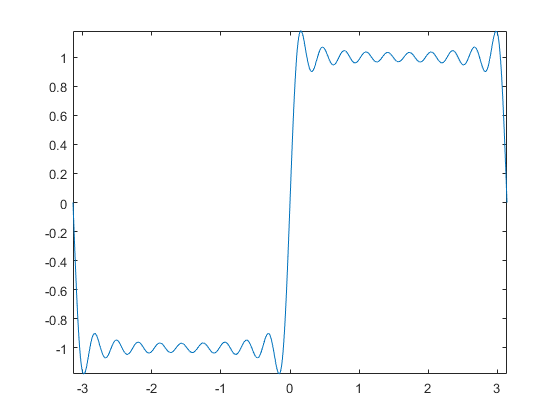
\includegraphics{problem_3_12_hw_5.png}
    \caption{$f_{20}(x)$ plotted on $[-\pi,\pi]$.}
    \label{fig:my_label}
\end{figure}
\pagebreak

\begin{figure}[h!]
    \centering
    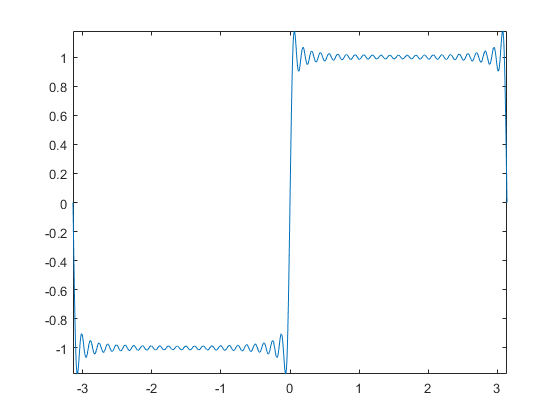
\includegraphics{problem_3_13_hw_5.png}
    \caption{$f_{50}(x)$ plotted on $[-\pi,\pi]$.}
    \label{fig:my_label}
\end{figure}
\end{solution}

\clearpage
\newpage
\paragraph{Matlab Code:}

\lstset{language=Matlab,%
    %basicstyle=\color{red},
    breaklines=true,%
    morekeywords={matlab2tikz},
    keywordstyle=\color{blue},%
    morekeywords=[2]{1}, keywordstyle=[2]{\color{black}},
    identifierstyle=\color{black},%
    stringstyle=\color{mylilas},
    commentstyle=\color{mygreen},%
    showstringspaces=false,%without this there will be a symbol in the places where there is a space
    numbers=left,%
    numberstyle={\tiny \color{black}},% size of the numbers
    numbersep=9pt, % this defines how far the numbers are from the text
    emph=[1]{for,end,break},emphstyle=[1]\color{red}, %some words to emphasise
    %emph=[2]{word1,word2}, emphstyle=[2]{style},    
}

\lstinputlisting{math_545_homework_5.m}

\end{document}



